\chapter{Architettura Software dello strumento}
\label{capitolo4}
\thispagestyle{empty}

\textit{In questo Capitolo verrà descritta l’architettura software dello strumento realizzato. Inizialmente verrà analizzato l’ambiente di sviluppo software. Successivamente verrano mostrati i principi alla base della programmazione per microcontrollore e FPGA. Infine, verranno illustrate e descritte le funzionalità implementate su FPGA e microcontrollore.}

\section{Ambiente di sviluppo LabVIEW}
L'ambiente di sviluppo scelto per questo lavoro di Tesi è NI LabVIEW.

LabVIEW, abbreviazione di \textit{Laboratory Virtual Instrumentation Engineering Workbench}, è l'ambiente di sviluppo integrato per il linguaggio di programmazione visuale di \textit{National Instruments}: il linguaggio G (\textit{G-Language}, abbreviazione di \textit{Graphical Language}).

La differenza sostanziale tra il linguaggio G e i linguaggi tradizionali risiede nella sintassi e nel controllo del flusso di programma:
\begin{itemize}
	\item \underline{Sintassi}: La sintassi del linguaggio G non è scritta ma grafica. 
	\item \underline{Controllo del flusso di programma}: Nei linguaggi tradizionali di tipo testuale, l'ordine di esecuzione delle istruzioni che costituiscono il codice del programma è determinato, a meno di ottimizzazioni portate dal compilatore, dall'ordine in cui le istruzioni sono scritte all'interno del codice stesso. Mentre, nel linguaggio G, l'ordine di esecuzione è stabilito dal "flusso di dati", ovvero ciascuna istruzione viene eseguita non appena sono disponibili i suoi dati di ingresso.
\end{itemize}

I programmi generati da LabVIEW prendono il nome di "strumenti virtuali" (\textit{Virtual Instrument}, VI). Un programma VI è composto da due parti fondamentali: il Pannello frontale (\textit{Front Panel}) e il Diagramma a blocchi funzionale (\textit{Block Diagram}).

\begin{figure}
\centering
\subfigure[Front Panel]
{\label{esempiolva}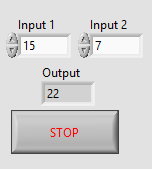
\includegraphics[scale=.8]{cap4/esempiolvaimg}}
\hspace{5mm}
\subfigure[Block Diagram]
{\label{esempiolvb}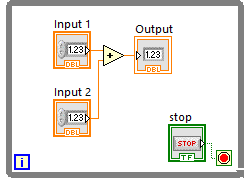
\includegraphics[scale=.8]{cap4/esempiolvbimg}}
\caption{Esempio di LabVIEW VI che calcola la somma di due numeri in virgola mobile}\label{esempiolv}
\end{figure}

Il pannello frontale è l'interfaccia utente del VI. Esso permette di definire ed introdurre tutte le grandezze di ingresso (input del programma) e tutte le grandezze in uscita (valori delle misure, grafici, ecc.). Si realizza con controlli e indicatori, che costituiscono, rispettivamente, i terminali interattivi d'ingresso e d'uscita.
 
Lo schema a blocchi è il diagramma di flusso che rappresenta il codice sorgente, in formato grafico. Esso è composto da due elementi distinti: i \textit{nodi} e i \textit{collegamenti}. I \textit{nodi} sono gli elementi di elaborazione, mentre i \textit{collegamenti} sono i fili che uniscono i vari nodi e permettono lo scambio di informazione ovvero il flusso dei dati.

\begin{figure}  
  \begin{center}
    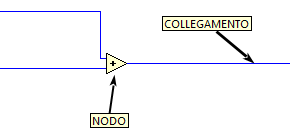
\includegraphics[scale=0.5]{cap4/nodocoll}
    \caption{Esempio di Nodo e di Collegamento}
    \label{nodocoll}
  \end{center}
\end{figure}

Le istruzioni, definite in fase di stesura del codice mediante il linguaggio grafico, vengono tradotte in modo trasparente in linguaggio C e successivamente compilate.

Le caratteristiche principali che hanno portato alla scelta di LabVIEW e del linguaggio G sono:
\begin{itemize}
	\item LabVIEW un ambiente di sviluppo orientato fortemente all'acquisizione dati e all'analisi ed elaborazione numerica di segnali
	\item Il linguaggio G possiede un parallelismo intrinseco che è facile da utilizzare grazie alla metodologia di scrittura grafica dei programmi. La programmazione parallela consente di raggiungere elevate prestazioni di calcolo, specialmente nella programmazione per FPGA
	\item LabVIEW include al suo interno una serie di librerie per l'analisi dei segnali disponibili anche per la compilazione su FPGA che ha notevolmente accelerato il processo di sviluppo del codice
	\item LabVIEW è l'unico linguaggio di programmazione ufficialmente supportato dalla scheda di prototipazione scelta (vedi Capitolo \ref{capitolo3})
\end{itemize}

\section{Sistema Real-Time e FPGA}
Come già accennato nel Capitolo precedente, lo scopo di questo lavoro di Tesi è la realizzazione di un prototipo di un misuratore di distanza basato sull'utilizzo di tecnologie FPGA e microcontrollore.

\subsection{Programmazione del microcontrollore}
	Lo sviluppo di codice per un sistema \textit{embedded} basato su microcontrollore si può suddivere in due approcci:
	\begin{enumerate}
		\item \underline{Bare-metal approach}: consiste in una programmazione a basso livello dove il codice viene caricato direttamente sul dispositivo hardware (in questo caso microontrollore).  Questo approccio è utilizzato quando la complessità del sistema non è elevata. Pertanto garantisce un occupazione di memoria molto piccola (\textit{memory footprint}). Un grosso svantaggio è la poca flessibilità ai cambiamenti di specifiche.
		\item \underline{Real-time Operating System approach}: consiste in una programmazione basata sul supporto di un sistema operativo \textit{Real-Time}. Questo approccio sfrutta tutti i vantaggi dell'utilizzo di un OS (programmazione \textit{multi-thread}, astrazione dell'hardware, ecc...).
	\end{enumerate}
	
	Per i motivi sopracitati si è scelto di sfruttare i vantaggi dell'utilizzo di un sistema Real-Time. Nel paragrafo successivo verrano trattate le caratteristiche dei sistemi Real-Time, i sistemi operativi Real-Time e in particolare il sistema operativo in uso sulla scheda di prototipazione scelta.
	
\begin{figure}  
  \begin{center}
    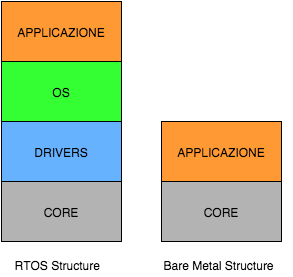
\includegraphics[scale=0.7]{cap4/baremetalrtos}
    \caption{Schema di funzionamento dei due approcci: RTOS e Bare-metal}
  \end{center}
\end{figure}
	
\subsubsection{Sistema Real-Time}

Un \textit{Real-Time System} (RTS) è un sistema in cui la correttezza del comportamento del sistema non dipende solo dall'esattezza dei risultati dei calcoli, ma anche dall'istante temporale in cui questi risultati vengono prodotti \cite{kopetzrt}.

Un'applicazione Real-Time è costituita da un insieme di \textit{task} (compiti) cooperanti. Ogni task possiede una scadenza temporale (\textit{deadline}) entro la quale deve completare la sua esecuzione. Le deadline possono essere di tre tipologie:
\begin{enumerate}
	\item \underline{Hard-deadline}: Una deadline si dice \textit{hard} se le conseguenze della sua violazione portano a un fallimento del sistema.
	\item \underline{Firm-deadline}: Una deadline si dice \textit{firm} se i risultati del corrispondente \textit{task} cessano di essere utili non appena la scadenza viene violata \cite{259423}. Gli effetti della sua violazione non sono catastrofici ma degradano le prestazioni del sistema.
	\item \underline{Soft-deadline}: Una deadline si dice \textit{soft} se l'utilità dei risultati prodotti dal task diminuiscono nel tempo dopo la scadenza. Gli effetti della sua violazione non produce problemi.
\end{enumerate}

\paragraph{Sistema Operativo Real-Time}
Un sistema operativo real-time (abbreviato RTOS, \textit{Real-Time Operating System}) è un sistema operativo specializzato al supporto di applicazioni Real-Time.

Gli RTOS sono solo un elemento di un più complesso sistema real-time. I loro obiettivi sono quelli di fornire un ambiente comodo per riuscire a sviluppare efficacemente l'applicazione gestendo al meglio le risorse, ma soprattutto rispettando i vincoli temporali imposti \cite{fornacia}.

Gli aspetti principali che differenziano un RTOS rispetto a un normale sistema operativo sono:
\begin{itemize}
	\item \underline{Determinismo}: è in grado di svolgere operazioni entro limiti di tempo prefissati.
	\item \underline{Latenza}: La latenza è l'intervallo di tempo che intercorre fra il momento in cui arriva l'input al sistema ed il momento in cui è disponibile il suo output. Nei RTOS viene posto un limite massimo al tempo di latenza per garantire il determinismo.
	\item \underline{Controllo utente}: Il controllo utente è più ampio rispetto ai normali OS. Il programmatore ha un controllo più fine sulle priorità, sull'uso di memoria dei processi e sulla gestione degli interrupt.
	\item \underline{Affidabilità}: Gli RTOS sono progettati in modo da far fronte ai fallimenti del sistema, cercando di preservare quante più informazioni possibili. Contrariamente ai normali OS, non si notifica solo il guasto all'utente ma si cerca di risolvere il problema.
\end{itemize}

Lo scheduling nei RTOS è solitamente semplificato: politiche FIFO o \textit{Round-Robin}. \'E comune l'utilizzo della prelazione (\textit{preemption}) e delle priorità.

I Sistemi Operativi Real-Time più comuni in commercio sono: \textit{VxWorks}, \textit{LynkOS} e \textit{Windows CE}. Esistono anche RTOS gratuiti e \textit{open-source} come: \textit{FreeRTOS} e \textit{eCos}.

L'RTOS presente sulla scheda di prototipazione utilizzata è \textit{VxWorks}.


\subparagraph{VxWorks}
\textit{VxWorks}, prodotto da \textit{WindRiver}, è il più famoso sistema operativo per applicazioni real-time; la notorietà è dovuta al suo utilizzo da parte della NASA nelle sonde spaziali \cite{fornacia}.

La struttura del sistema operativo è basata su \textit{micro-kernel}. Il \textit{micro-kernel}, contrariamente al kernel monolitico, fornisce solo le funzionalità strettamente necessarie alla gestione dei processi. Le funzionalità accessorie, come ad esempio la gestione di rete, sono rese disponibili da librerie esterne al kernel. Questa soluzione offre un ristretto utilizzo di memoria e libertà al progettista di personalizzare il sistema con le funzionalità prescelte.

\begin{figure}  
  \begin{center}
    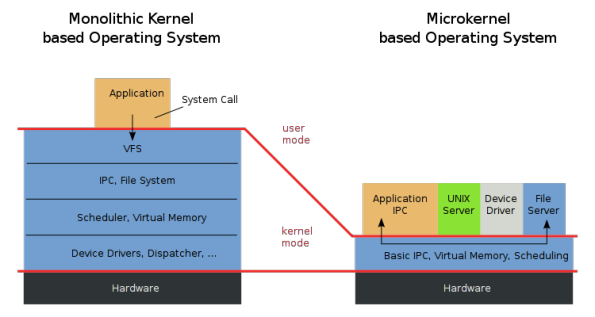
\includegraphics[scale=0.5]{cap4/microvsmono}
    \caption{Confronto tra kernel monolitico e micro-kernel}
  \end{center}
\end{figure}

Lo scheduling utilizzato da \textit{VxWorks} utilizza la politica Round-Robin con diritto di prelazione e priorità. I task con priorità più elevata vengono eseguiti per primi e nel caso di task con la stessa priorità l'esecuzione è Round-Robin.
\begin{figure}  
  \begin{center}
    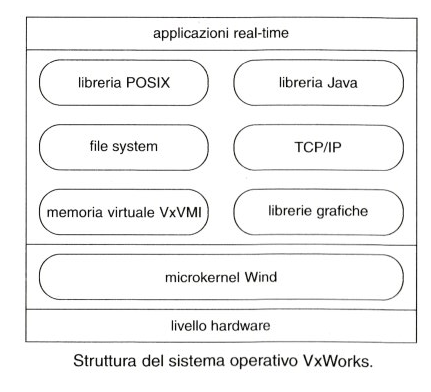
\includegraphics[scale=0.5]{cap4/vxworks}
    \caption{Struttura del sistema operativo VxWorks}
  \end{center}
\end{figure}

La comunicazione tra processi può sfruttare una serie di meccanismi predefiniti come: strutture dati condivisibili (es. variabili globali), semafori e code.

Maggiori informazioni sul sistema operativo \textit{VxWorks} si possono trovare sul sito web dello sviluppatore \cite{sitevxworks}.

\paragraph{LabVIEW Real-Time}
Per lo sviluppo dell'architettura Real-Time di questo lavoro di Tesi è stato utilizzato il modulo software LabVIEW Real-Time.

NI LabVIEW \textit{Real-Time Module} è un componente aggiuntivo di LabVIEW utilizzato per la creazione di applicazioni Real-Time in esecuzione su dispositivi hardware \textit{embedded}.

\begin{figure}  
  \begin{center}
    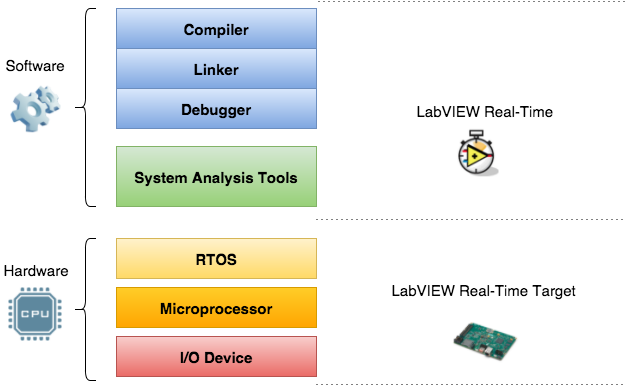
\includegraphics[scale=0.5]{cap4/lvrt}
    \caption{Struttura del modulo LabVIEW Real-Time}
    \label{labviewrt}
  \end{center}
\end{figure}

\begin{figure}  
  \begin{center}
    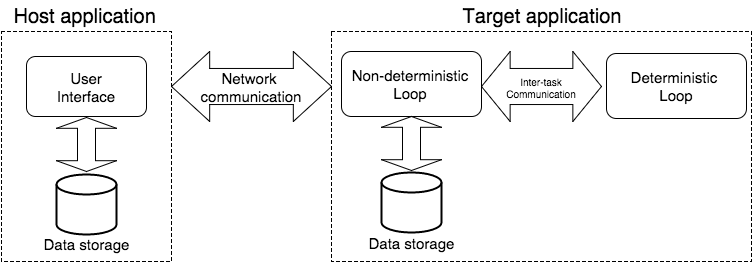
\includegraphics[scale=0.4]{cap4/lvrtvi}
    \caption{Architettura software di un applicazione LabVIEW Real-Time}
    \label{labviewrtvi}
  \end{center}
\end{figure}

La Figura \ref{labviewrtvi} mostra l'architettura software di base di un'applicazione Real-Time sviluppata in LabVIEW. Un applicazione LabVIEW Real-Time si divide in due parti: applicazione \textit{host} e \textit{target}.

L'applicazione \textit{host}, eseguita sul computer host, ha il compito di interfacciarsi con l'utente e comunicare con l'applicazione target. 

L'applicazione \textit{target}, invece, è l'applicazione Real-Time eseguita dal microprocessore del target computer. Nel nostro lavoro di Tesi il target computer è la scheda di prototipazione \textit{Single Board RIO 9636} ampiamente descritta nel Capitolo \ref{capitolo3}.

L'applicazione \textit{target} è composta da processi. Un processo è un insieme di operazioni che si ripetono iterativamente nel tempo consumando una precisa quantità di tempo del microprocessore (\textit{deadline}).
\begin{figure}
\centering
\subfigure[Timed Loop (Deterministico)]
{\label{timedloop}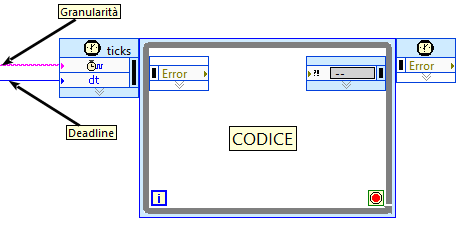
\includegraphics[scale=.5]{cap4/timed}}
\hspace{5mm}
\subfigure[While Loop (Non deterministico)]
{\label{whileloop}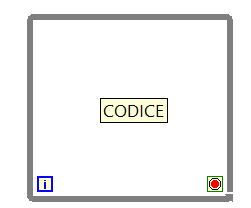
\includegraphics[scale=.5]{cap4/while}}
\caption{Cicli deterministici e non-deterministici}
\end{figure}

In LabVIEW un processo è rappresentato graficamente da un ciclo (\textit{loop}) in cui sono racchiuse le operazioni da eseguire. Essi si suddividono in due categorie:
\begin{enumerate}
	\item \underline{Deterministici} (\textit{Deterministic loop/process}): processi \textit{Hard-deadline}. Sono rappresentati graficamente da Timed Loop (Figura \ref{timedloop}).
	\item \underline{Non Deterministici} (\textit{Non-deterministc loop/process}): processi \textit{Soft-deadline}. Sono rappresentati graficamente da While Loop (Figura \ref{whileloop}).
\end{enumerate}

\subsection{Progettazione e programmazione dell'FPGA}
FPGA, ampiamente descritto nel Capitolo \ref{capitolo3}, è un dispositivo logico le cui funzionalità sono programmabili via software.

Una delle tecniche più utilizzate per specificare la funzionalità di un dispositivo logico riprogrammabile consiste nell'uso di un linguaggio di descrizione dell'hardware (HDL, \textit{Hardware Description Language}). Esistono anche tecniche che utilizzano strumenti grafici (EDA, \textit{Electronic Design Automation}) per definire lo schema circuitale.

L'HDL è adatto alla progettazione di grandi architetture perché permette di definire numericamente gli elementi circuitali. Tuttavia, l'utilizzo dello schema circuitale permette una lettura dell'architettura più chiara rispetto all'HDL.

\subsubsection{Linguaggi di descrizione dell'Hardware (HDL)}
Un linguaggio per la descrizione dell'hardware o HDL (\textit{Hardware Description Language}) è uno strumento di supporto alla progettazione dei circuiti digitali che ha lo scopo di cogliere gli aspetti funzionali e architetturali di un sistema \cite{fornacia}.

La principale caratteristica di un HDL è la concorrenzialità: ovvero le diverse parti di un codice HDL una volta tradotte in un circuito elettronico, funzionano contemporaneamente, in quanto dispongono di hardware dedicato; al contrario, di un linguaggio software.

Esistono due linguaggi di descrizione dell'hardware attualmente utilizzati: VHDL e Verilog. La toolchain utilizzata per lo sviluppo di questo progetto, che verrà descritta in seguito, fa uso del linguaggio VHDL.

\paragraph{VHDL}
VHDL è l'acronimo di \textit{VHSIC Hardware Description Language}, dove VHSIC è un altro acronimo: \textit{Very High-Speed Integrated Circuits} \cite{storeyelet}.

La metodologia di programmazione di questo linguaggio si basa sul concetto di componente. Il componente è un'unità funzionale e il sistema è rappresentato da una rete gerarchica di componenti.

Le principali fasi di progettazione sono due:
\begin{itemize}
	\item \underline{Entity}: Un entity definisce l'interfaccia di un componente, in particolare le porte di comunicazione e altri parametri come: tempi di ritardo, larghezza del bus, ecc.
	\item \underline{Architecture}: L'architecture definisce la funzionalità svolta dal componente. Per questa fase vengono usati di solito due stili:
	\begin{enumerate}
		\item \underline{Behavioural}: La relazione funzionale ingressi-uscite è espressa tramite un algoritmo. Vengono utilizzati i costrutti noti dei linguaggi di programmazione software come \textit{if-then-else}.
		\item \underline{Structural}: Non viene evidenziata la funzionalità ma la struttura interna del componente. La struttura è formata da componenti di basso livello (segnali, elementi di memoria, ecc.) ed i loro collegamenti (RTL, \textit{Register Transfer Level}).
	\end{enumerate} 
\end{itemize}

VHDL è diventato lo standard IEEE $1076$ nel $1987$. \'E stato aggiornato nel $1993$ ed è conosciuto oggi come "standard IEEE $1076$ $1993$" \cite{545676}. 
		
\subsubsection{Sintesi Hardware}
La sintesi Hardware è il processo di compilazione che trasforma una specifica hardware, espressa in HDL o con schema circuitale, in un file di configurazione per il dispositivo hardware riprogrammabile.

Le principali fasi della sintesi hardware sono:
\begin{itemize}
	\item \underline{Translation}: Molti software per la sintesi hardware consentono al programmatore di poter scrivere la specifica hardware in diversi modi (HDL o schema circuitale). La prima fase della compilazione consiste nel combinare e tradurre le diverse specifiche in un'unica specifica completa.
	\item \underline{Functional simulation}: Questa fase consiste nella simulazione dell'architettura progettata. Questo processo verifica la correttezza logica del circuito senza considerare i vincoli temporali.
	\item \underline{Optimisation}: Dopo che l'architettura è stata valutata logicamente corretta, viene effettuata un ottimizzazione automatica al fine di semplificarne l'implementazione. Le ottimizzazioni più comuni sono le semplificazioni aritmetico-logiche.
	\item \underline{Mapping}: L'architettura ottimizzata viene distribuita sulle risorse disponibili del dispositivo hardware. Il processo è molto impegnativo nel caso di programmazione FPGA perché esistono svariati modi per tracciare le interconnessioni.
	\item \underline{Place and route}: La configurazione risultante dal processo di Mapping viene sottoposta ad una dettagliata simulazione temporale. Questa fase verifica che l'architettura realizzata rispetti i vincoli temporali sul dispositivo hardware reale.
	\item \underline{Configuration data}: Se i risultati della simulazione temporale sono soddisfacenti, viene generato un file di configurazione chiamato \textit{bitfile}. Il \textit{bitfile} contiene tutte le informazioni necessarie per configurare correttamente l'architettura progettata sul dispositivo hardware programmabile.
\end{itemize}

\begin{figure}  
  \begin{center}
    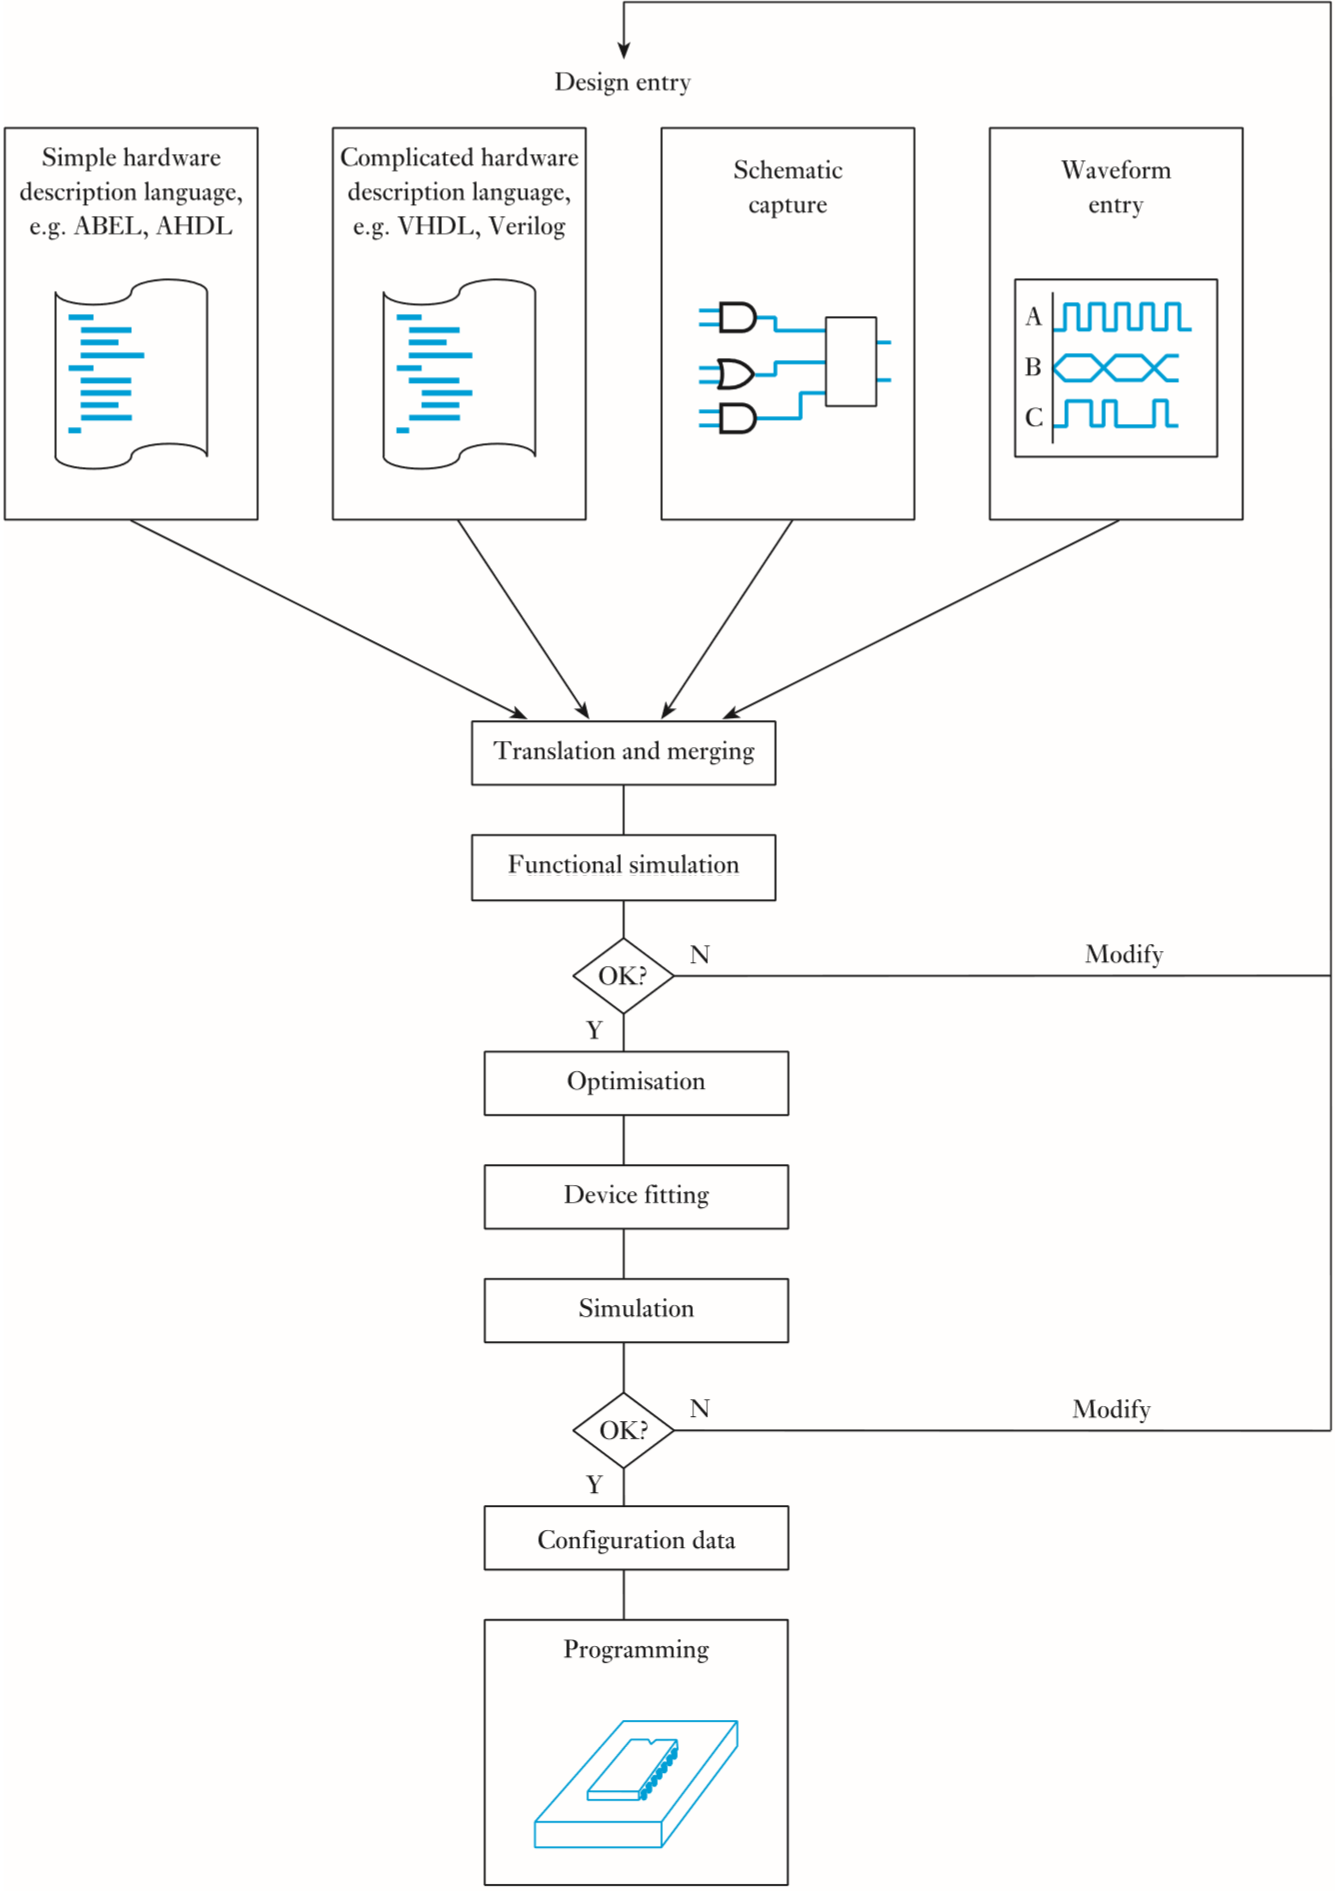
\includegraphics[scale=0.35]{cap4/sinthw}
    \caption{Sintesi hardware}
  \end{center}
\end{figure}
		
\subsubsection{High-Level Synthesis (HLS)}
\textit{High-level synthesis} (HLS), in italiano Sintesi ad alto livello, è un processo automatizzato di compilazione che interpreta una descrizione algoritmica di un desiderato comportamento e crea l'hardware digitale che implementa tale comportamento \cite{Coussy:2008:HSA:1457713}.

La descrizione algoritmica del comportamento è espressa con linguaggi di alto livello come C, infatti è talvolta chiamata \textit{C-Synthesis}. Nella pratica, gli strumenti di compilazione HLS convertono codice C o C-like in un linguaggio di descrizione dell'hardware (HDL), come VHDL o Verilog. 

La scrittura di codice di alto livello permette al progettista di concentrarsi solo sull'aspetto funzionale dell'architettura. Quindi, ad un livello di astrazione più alto, sono necessari meno dettagli per la descrizione di un comportamento. Ad esempio, non si ha bisogno di preoccuparsi dei dettagli implementativi come gerarchie, processi, temporizzazioni, ecc.. come avviene per i linguaggi di descrizione dell'hardware. Questo rende la descrizione molto più facile da scrivere, riducendo notevolmente il rischio di errori e il tempo di testing. 

La sintesi HLS è costituita da una serie di attività e diversi tool HLS eseguono queste attività in ordine diverso utilizzando algoritmi differenti. Altri tool HLS combinano alcune di queste attività e le eseguono iterativamente al fine di convergere verso la soluzione desiderata \cite{eetimes}.

Di seguito vengono elencati i passi principali del processo di sintesi di alto livello:
\begin{enumerate}
	\item \underline{Algorithm optimization}: Nella prima fase, vengono eseguite ottimizzazioni del codice comunemente usate nei compilatori dei linguaggi ad alto livello come ad esempio: \textit{Common Subexpression Elimination} (CSE), \textit{Constant Propagation}, ecc.
	\item \underline{DataFlow Graph analysis}: Vengono analizzate le operazioni aritmetico-logiche e le dipendenze tra i dati. Il risultato di questa analisi si traduce nella costruzione di un grafo chiamato \textit{DataFlow Graph} (DFG). Il grafo rappresenta le dipendenze dei dati e indica l'ordine di esecuzione delle operazioni.
	\item \underline{Resource allocation}: Dopo che il DFG è stato creato, ogni operazione aritmetico-logica viene attribuita ad una risorsa hardware. La risorsa hardware corrisponde ad un'implementazione fisica dell'operatore aritmetico-logico. Ogni operatore può avere più implementazioni hardware, ciascuna con differenti caratteristiche di area/ritardo/latenza. Queste risorse sono selezionate da una libreria tecnologica che contiene tutte le implementazioni disponibili.
	\item \underline{Scheduling}: Questa fase introduce il concetto di tempo e di parallelismo. Lo scheduling prende le operazioni descritte nel DFG e decide quando (in quale ciclo di clock) saranno eseguite \cite{bluebook}.
	\item \underline{Module binding}: Il module binding è la fase che assegna le operazioni aritmetico-logico a specifiche istanze di risorse hardware. Questa fase si basa sulle tipologie e le quantità di risorse hardware scelte nella fase di resource allocation.
	\item \underline{Register binding}: I registri di memoria sono necessari quando i valori prodotti in un ciclo di clock vengono utilizzati in un ciclo di clock differente. La fase del Register Binding consiste nell'allocare i registri necessari a conservare questi valori. In questa fase viene effettuata l'analisi del ciclo di vita di ogni valore allo scopo di poter utilizzare lo stesso registro fisico per memorizzare valori diversi in istanti di tempo diversi.
	\item \underline{Output processing}: I risultati prodotti dai passi precedenti vengono tradotti in codice HDL.
\end{enumerate}

Per i motivi esposti all'inizio del paragrafo, abbiamo scelto di utilizzare un'ambiente di sviluppo che permettesse di sfruttare i benefici della sintesi ad alto livello. L'ambiente di sviluppo utilizzato per la programmazione della scheda FPGA è descritto nel paragrafo successivo.

\begin{figure}  
  \begin{center}
    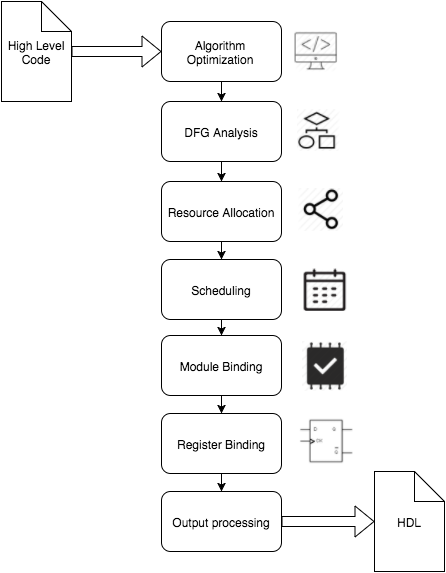
\includegraphics[scale=0.4]{cap4/hls}
    \caption{High Level Synthesis}
  \end{center}
\end{figure}
		
\subsubsection{LabVIEW FPGA}
Per lo sviluppo dell'architettura FPGA di questo lavoro di Tesi è stato utilizzato il modulo software LabVIEW FPGA. NI LabVIEW \textit{FPGA Module} è un componente aggiuntivo di LabVIEW utilizzato per sviluppare applicazioni per FPGA.

Questo ambiente di sviluppo compila ed esegue il codice LabVIEW sul dispositivo FPGA. Il processo di compilazione automatica è suddiviso in tre fasi:
\begin{enumerate}
	\item \underline{High-Level Synthesis}: Il codice di alto livello LabVIEW viene tradotto in codice VHDL
	\item \underline{Hardware Synthesis}: Il codice VHDL, prodotto nel passo precedente, viene tradotto dal compilatore \textit{Xilinx ISE}. \textit{Xilinx ISE Compiler} è uno strumento software prodotto da \textit{Xilinx} che effettua la sintesi hardware di codice HDL. Il risultato finale di questa fase è l'FPGA \textit{bitfile}.
	\item \underline{Bitfile download}: Il \textit{bitfile} generato dal compilatore di \textit{Xilinx} viene caricato ed eseguito sull'FPGA.
\end{enumerate}

\begin{figure}  
  \begin{center}
    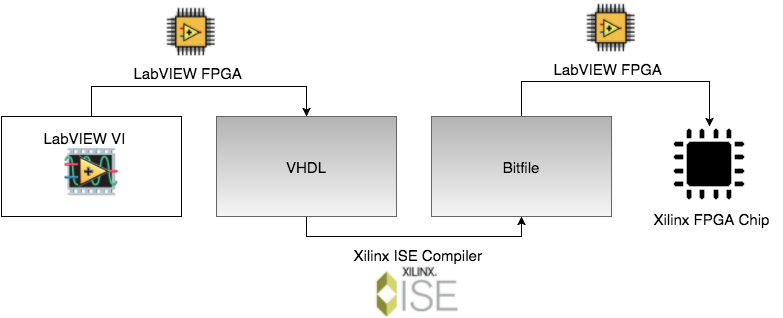
\includegraphics[scale=0.4]{cap4/fpgalv}
    \caption{Processo di compilazione LabVIEW FPGA}
  \end{center}
\end{figure}

Al contrario del microprocessore, non esiste alcun sistema operativo sul chip FPGA, ma LabVIEW FPGA offre comunque la possibilità di controllare ingressi e uscite attraverso un applicazione host.
		
\section{Analisi teorica degli algoritmi implementati}
In questo paragrafo verranno introdotti i concetti fondamentali alla base dei principali algoritmi utilizzati nell'ambito dello sviluppo del firmware dell'interferometro.

Gli algoritmi utilizzati sono:
\begin{itemize}
	\item Fast Fourier Transform (FFT)
	\item Interpolated Fast Fourier Transform (IFFT)
	\item Calcolo della distanza assoluta
\end{itemize}

\subsection{Fast Fourier Transform (FFT)}
Prima di illustrare il funzionamento dell'algoritmo di FFT, è bene richiamare alcuni concetti sull'analisi in frequenza dei segnali.

I principali metodi di analisi dei segnali di misura sono l'analisi nel dominio del tempo e nel dominio della frequenza. I due approcci sono tra loro intercambiabili, ovvero, sotto opportune condizioni, nessun informazione viene persa nel passare da un dominio all'altro. 

Lo strumento matematico che consente di trasferire lo studio dei segnali dal dominio del tempo al dominio della frequenza è la trasformata di \textit{Fourier}.

Il campionamento di un segnale analogico $x(t)$ consiste nel prenderne solo i valori $x(iT_s)$ in corrispondenza di istanti ben precisi $iT_s$ detti istanti di campionamento. 
Il campionamento ideale consiste nel moltiplicare il segnale $x(t)$ per il treno di impulsi $s(t)$:
\begin{equation}
	x_s(t)=x(t) s(t) = \sum_{n=-\infty}^{+\infty} x(nT_s) (\delta (t-nT_s))
\end{equation}
\begin{figure}  
  \begin{center}
    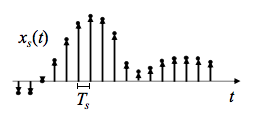
\includegraphics[scale=0.6]{cap4/trenoimp}
    \caption{Segnale campionato con treno di impulsi}
  \end{center}
\end{figure}

Lo spettro in frequenza del segnale campionato è dato dalla Trasformata di Fourier Tempo Discreta (DTFT), espressa dall'equazione: 
\begin{equation}
	X(e^{j\omega}) = \sum_{n=-\infty}^{+\infty} x(n)e^{-j\omega n}
\end{equation}
dove $x(n)$ indica la sequenza infinita di campioni in ingresso e $\omega$ la pulsazione continua espressa in radianti.

Considerando, invece, una sequenza finita $x[n]$ di lunghezza $N$, a cui corrisponde la DTFT $X(e^{j\omega})$, è possibile definire la Trasformata di Fourier Discreta (DFT) come la sequenza di $N$ campioni:
\begin{equation}
	X(k)=X(e^{j\omega}) |_{\omega = \frac{2 \pi k}{N}} = \sum_{n=0}^{N-1} x(n)e^{-j \frac{2 \pi}{N} k n}
	\label{dfteq}
\end{equation}

La DFT è costituita da un campionamento delle pulsazioni della DTFT con passo di quantizzazione $\frac{2 \pi}{N}$ dove ogni pulsazione quantizzata:
\begin{equation}
	\omega _k = \frac{2 \pi k}{N} 
\end{equation}
con:
$$0 \leq k \leq N-1$$
viene chiamata \textit{bin}. Si nota che lo spettro è calcolato unicamente per le frequenze di bin.

Per ottenere la sequenza $x[k]$ a partire dai campioni $x[n]$ è necessario uno sforzo computazionalmente considerevole (complessità quadratica $O(N^2)$). Esso è dovuto all'elevato numero di operazioni di moltiplicazione e addizione presenti nel calcolo della DFT. Per tale motivo, sono stati realizzati algoritmi che riducono notevolmente il numero di operazioni necessarie rendendo il costo computazionale meno cospicuo.

Questi algoritmi hanno complessità $O(NlogN)$ e prendono il nome di 
\textit{Fast Fourier Transform (FFT) algorithm}.

L'algoritmo FFT più diffuso è il \textit{Cooley-Tukey algorithm} che si basa sul principio di \textit{divide et impera}. L'algoritmo decompone ricorsivamente ad ogni passo la DFT in dimensioni più piccole.

Ai fini della trattazione dell'algoritmo di \textit{Cooley-Tukey} si introduce il \textit{twiddle factor} $W_N = e^{-j \frac{2 \pi}{N}}$ riscrivendo l'equazione \ref{dfteq} come:
\begin{equation}
	X(k)=\sum_{n=0}^{N-1} x(n)W_N^{kn} 
	\label{dfteq2}
\end{equation}

L'uso più conosciuto dell'algoritmo è di dividere ricorsivamente la DFT in due parti da $\frac{N}{2}$ ad ogni passo. Esso è quindi ottimizzato solo per dimensioni che siano potenze di due, ma in generale può essere utilizzato con qualsiasi fattorizzazione.

Se consideriamo come numero di campioni $N$ della DFT una potenza di due possiamo riscrivere l'equazione \ref{dfteq2} separando i termini di indice pari e di indice dispari ottenendo così l'equazione:
\begin{equation}
\begin{split}
	X(k) &= \sum_{n\ pari} x(n)W_{N}^{kn} + \sum_{n\ dispari} x(n)W_{N}^{kn} \\
	&= \sum_{n=0}^{\frac{N}{2}-1} x(2n)W_{N}^{k2n} + \sum_{n=0}^{\frac{N}{2}-1} x(2n+1)W_{N}^{k(2n+1)}
\end{split}
\end{equation}
Essendo valida la relazione $W_N^2=W_{\frac{N}{2}}$, possiamo riscrivere la precedente equazione come:
\begin{equation}
\begin{split}
	X(k) &= \sum_{n=0}^{\frac{N}{2}-1} x(2n)W_{\frac{N}{2}}^{kn} + W_N^k \sum_{n=0}^{\frac{N}{2}-1} x(2n+1)W_{\frac{N}{2}}^{kn}\\
	&= X_1(k) + W_N^k X_2(k)
	\end{split}
\end{equation}
Siccome $X_1(k)$ e $X_2(k)$ sono periodiche di periodo $\frac{N}{2}$ ed è valida la relazione $W_N^{k + \frac{N}{2}}=-W_N^k$, possiamo riscrivere $X(k)$ come:
\begin{equation}
	X \left ( k+\frac{N}{2} \right ) =X_1(k) - W_N^k X_2(k)
\end{equation}

Dalle precedenti equazioni si osserva che il calcolo di $X_1(k)$ e $X_2(k)$ richiede $ \left ( \frac{N}{2} \right ) ^2$ moltiplicazioni mentre $W_N^k X_2(k)$ ne richiede solo $\frac{N}{2}$, ottenendo così $2 \left ( \frac{N}{2} \right ) ^2 + \frac{N}{2}$ moltiplicazioni per il calcolo di $X(k)$.

In confronto all'algoritmo di DFT vi è una riduzione di un fattore due del tempo di computazione $\left ( 2 \left ( \frac{N}{2} \right ) ^2 + \frac{N}{2} \right ) \approx \left ( \frac{N}{2} \right ) ^2  < N^2 $. 

Procedendo ricorsivamente e applicando la stessa tecnica di calcolo sulla DFT decomposta si ottengono $\log N$ iterazioni della procedura se $N$ è potenza di $2$. 
Pertanto, il calcolo della trasformata di un vettore con $N$ componenti richiama in maniera ricorsiva il calcolo della trasformata a due vettori con $\frac{N}{2}$ componenti in cui sono presenti $O(N)$ operazioni di somma e prodotto aggiuntive.  

Possiamo quindi definire, per il calcolo della complessità dell'algoritmo di FFT, il numero totale $T(N)$ delle operazioni necessarie per il calcolo della trasformata di Fourier di un vettore con $N$ componenti:
\begin{equation}
T(N)=
\left\{\begin{matrix}
 0, & N=1 \\ 
 2T \left ( \frac{N}{2} \right ), & N>1
\end{matrix}\right.
\end{equation}

la cui soluzione è $T(N)=O(N \log N )$.

Alla luce dei risultati appena esposti, possiamo concludere che l'algoritmo di FFT riduce notevolmente il tempo di computazione portando il numero di operazioni a $(\frac{N}{2}) \log N$.

\begin{algorithm}
\caption{Algoritmo di FFT}\label{alg:fft}
\begin{algorithmic}[1]
\Procedure{fft}{}
%% TODO: Cap4 Pseudocodice FFT
\EndProcedure
\end{algorithmic}
\end{algorithm}

Nel listato \ref{alg:fft} è mostrato lo pseudocodice dell'algoritmo di FFT.

Il calcolo della FFT è caratterizzato però da un problema che riguarda la valutazione finale dello spettro di frequenza: il calcolo della FFT si può considerare corretto solo se il segnale è periodico e l'analisi viene effettuata su un segnale campionato coerentemente, ovvero se si considerano un numero intero di periodi del segnale.
\begin{figure}  
  \begin{center}
    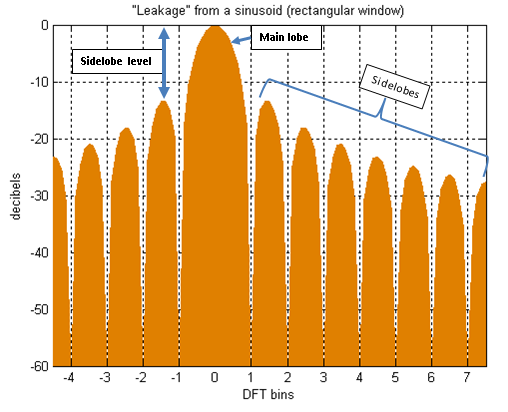
\includegraphics[scale=0.5]{cap4/spectleak}
    \caption{Spectral leakage}
    \label{spectleak}
  \end{center}
\end{figure}

Il calcolo del FFT su una finestra di osservazione non contenente un numero intero di periodi produce un allargamento e uno spostamento delle righe dello spettro di frequenza; questo fenomeno è chiamato \textit{spectral leakage} (dispersione spettrale, Figura \ref{spectleak}). 

Quindi, oltre a dover rispettare il teorema del campionamento di \textit{Nyquist}, bisogna prestare attenzione alla dispersione spettrale che causa \textit{aliasing} del segnale.

Applicare l'algoritmo di FFT direttamente alla sequenza campionata equivale ad usare una funzione di finestratura rettangolare, che pesa uniformemente i campioni.

Una soluzione che limita il fenomeno di \textit{spectral leakage} è l'utilizzo di una finestra rettangolare di troncamento contenente un numero intero di periodi. Tale soluzione non è sempre realizzabile perciò, nella pratica, si utilizza un'altra soluzione che consiste nel sostituire la finestra rettangolare con finestre che presentano una transizione graduale alle estremità. 

Pertanto, un importante aspetto da tenere in considerazione quando si esegue il calcolo della FFT di un segnale periodico campionato è l'operazione di finestratura \cite{31004}. 

Le finestre con transizione graduale alle estremità, chiamate anche \textit{smoothing window}, risolvono i problemi dovuti ad un campionamento non coerente. I problemi del campionamento non coerente si manifestano principalmente agli estremi della finestra di osservazione, dove si osservano discontinuità, quindi è ragionevole ipotizzare che se si potessero trascurare gli estremi e si potesse concentrare l'analisi sulla parte centrale della finestra di osservazione si otterrebbe uno spettro in frequenza più corretto. 

Pertanto, come già accennato, le \textit{smoothing window} pesano differentemente i vari campioni assumendo valore basso agli estremi e valore elevato nelle porzioni centrali della finestra.

Le \textit{smoothing window} sono divise tra finestre cosinusoidali e non cosinusoidali. Una delle più utilizzate è quella cosinusoidale di \textit{Hanning}.
\begin{figure}  
  \begin{center}
    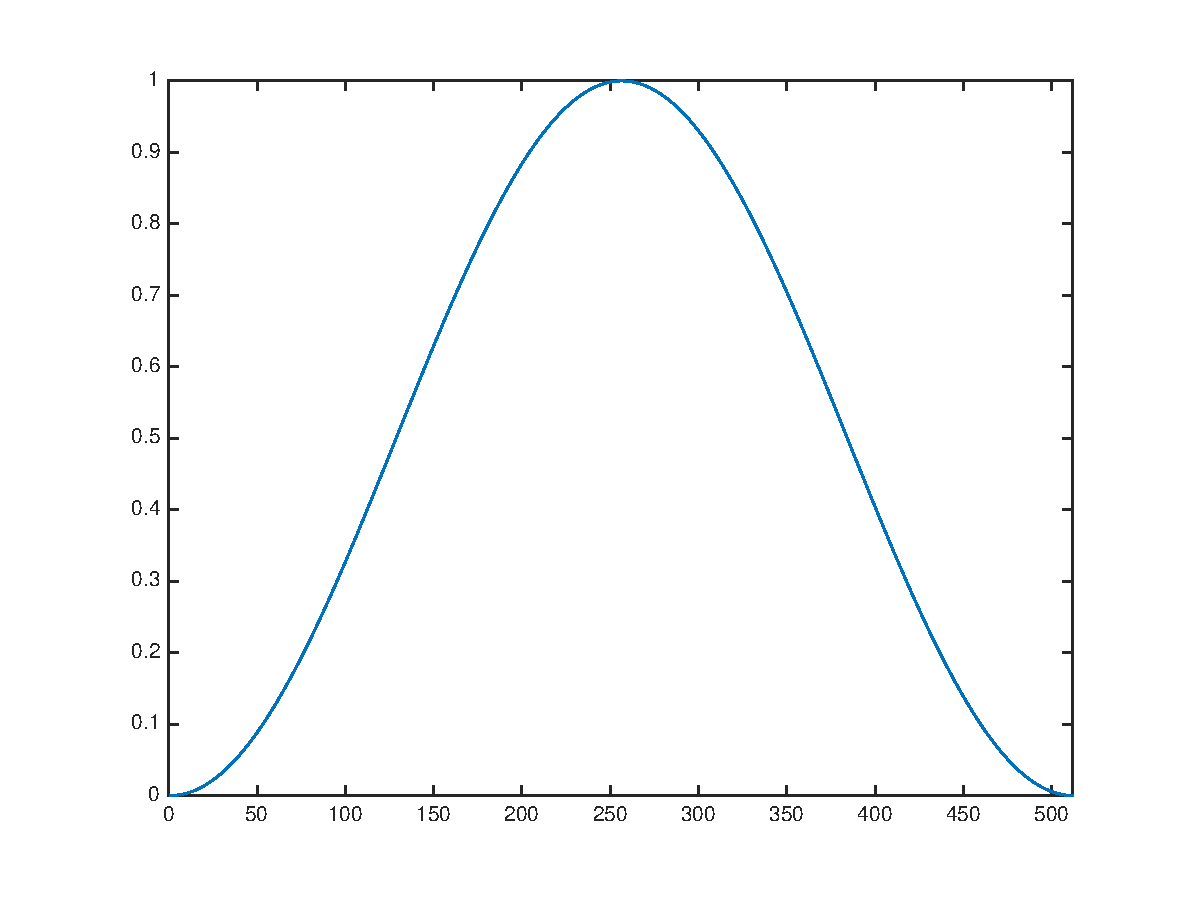
\includegraphics[scale=0.4]{cap4/hann}
    \caption{Finestra di Hanning}
    \label{hann}
  \end{center}
\end{figure}

La funzione peso della finestratura di \textit{Hanning} è definita dalla seguente relazione:
\begin{equation}
	w(n) = \frac{1}{2} \left [  1 - \cos \left ( \frac{2 \pi n}{N - 1} \right ) \right ]
\end{equation}
con:
$$ 0 \leq n \leq N-1 $$
ed è mostrata in figura \ref{hann}. La forma di questa finestra consente di eliminare la discontinuità del segnale agli estremi in caso di campionamento non coerente. 
\begin{figure}  
  \begin{center}
    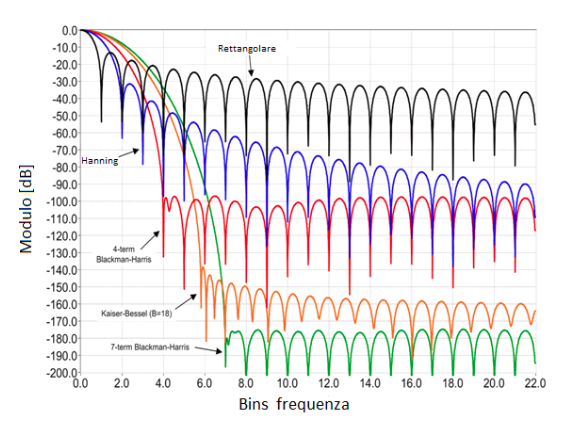
\includegraphics[scale=0.4]{cap4/smoothwins}
    \caption{Spectral leakage per diversi tipi di finestratura}
    \label{smoothwins}
  \end{center}
\end{figure}

Prima di eseguire l'algoritmo di FFT, quindi, ciascun campione della sequenza $x(n)$ viene moltiplicato per un coefficiente della funzione peso $w(n)$ della finestra. 
In figura \ref{smoothwins} è mostrato il confronto dello \textit{spectral leakage} per diversi tipi di finestratura. Emerge in modo chiaro dalla figura che l'utilizzo di \textit{smoothing window} riduce notevolmente il fenomeno di dispersione spettrale.

%% TODO Cap4 Dubbio se mettere questo pezzo qua
Concludendo, il parallelismo hardware intrinseco che si ottiene con l'FPGA è l'ideale per l'elaborazione numerica dei segnali in parallelo. Per tale motivo si è scelto di eseguire l'algoritmo di FFT su FPGA.

\subsection{Interpolated Fast Fourier Transform (IFFT)}
Come ampiamente descritto nel paragrafo precedente, per mezzo dell'algoritmo di FFT è possibile ricavare lo spettro di frequenza di un segnale. Lo spettro di frequenza ricavato è però discreto, pertanto le frequenze delle singoli componenti spettrali possono essere valutate dalla loro posizione nella spettro discreto con una risoluzione che dipende dal numero dei campioni \cite{31004}.

Se si campiona il segnale di ingresso con una frequenza $f_s$, si ottiene una risoluzione pari a:
\begin{equation}
	\Delta f = \frac{f_s}{N}
	\label{deltaf}
\end{equation}
dove $N$ è il numero dei campioni e $\Delta f$ è la distanza tra 2 \textit{bin} consecutivi.

Per migliorare la risoluzione del tono principale del segnale esistono algoritmi che utilizzano metodi di interpolazione.

%%TODO Cap4 riprendere da qui


\subsection{Calcolo della distanza assoluta}
	
\section{Architettura Software}

	\subsection{FPGA}
	
		\subsubsection{Implementazione software}
		
			\paragraph{Design pattern utilizzati}
		
				\subparagraph{Producer-consumer}
			
				\subparagraph{4-Wire Handshake}
			
			\paragraph{Fixed Point}
	
	\subsection{Microcontrollore}
	
		\subsubsection{Implementazione software}
	
	\subsection{Comunicazione tra FPGA e Microcontrollore}
